\section{Methodology: The Gated PINN Framework}\label{sec:method}

\subsection{Data Curation and Space-Weather Fusion}
The training corpus is built from Starlink TLE history across 2022--2026, covering both rising and peak Solar Cycle 25 conditions. For each anchor epoch $t_0$, we pair a future target epoch $t_0+\Delta t$ (typically near 24 h) and construct residual labels between propagated and target states:
\begin{equation}
[\mathbf{r}_{pred},\mathbf{v}_{pred}] = \mathrm{SGP4}(\mathrm{TLE}_{anchor},\Delta t),
\end{equation}
\begin{equation}
[\mathbf{r}_{true},\mathbf{v}_{true}] = \mathrm{SGP4}(\mathrm{TLE}_{target},0),
\end{equation}
\begin{equation}
\mathbf{y}=\left[\mathbf{r}_{true}-\mathbf{r}_{pred},\;\mathbf{v}_{true}-\mathbf{v}_{pred}\right].
\end{equation}
Feature vectors combine kinematics and drag proxies with exogenous weather drivers:
\begin{equation}
\mathbf{x}=\left[r_x,r_y,r_z,v_x,v_y,v_z,B^*,\dot{n},\Delta t,K_p,F_{10.7}\right].
\end{equation}
This formulation follows evidence that storm-time density and drag variability must be represented explicitly for resilient propagation \cite{oliveira2021current,li2025density}.

\begin{figure}[H]
\centering
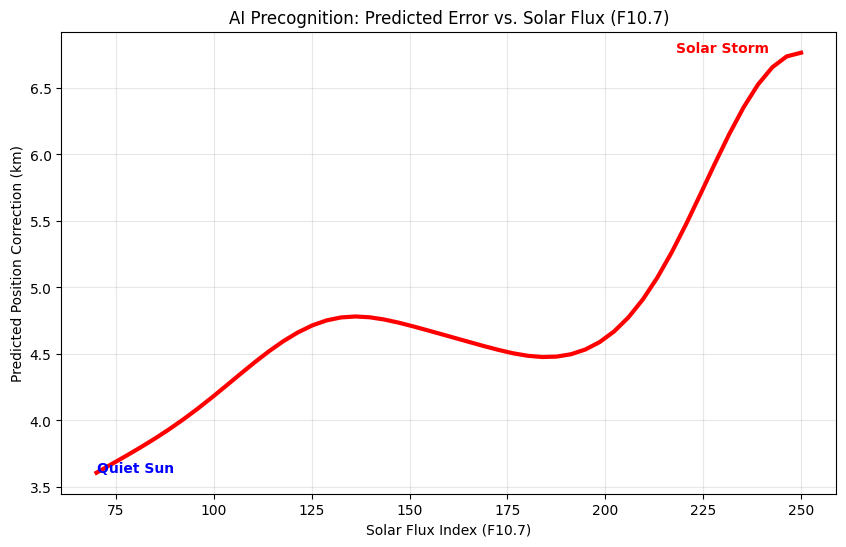
\includegraphics[width=\columnwidth]{figures/flux_anaysis.png}
\caption{Space-weather feature analysis used to condition storm-aware drag correction behavior.}
\label{fig:flux-analysis}
\end{figure}

\begin{figure}[H]
\centering
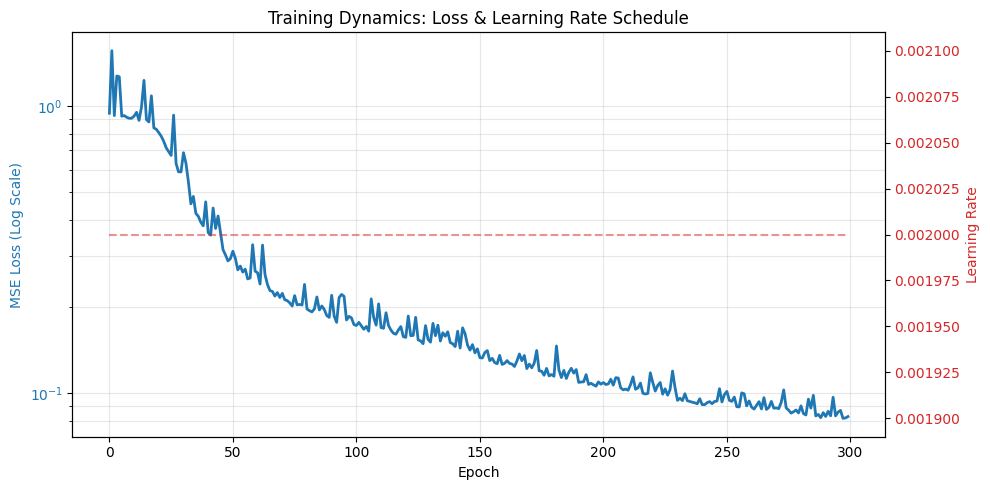
\includegraphics[width=\columnwidth]{figures/training.png}
\caption{Training dynamics of the G-PINN model across optimization epochs.}
\label{fig:training-curves}
\end{figure}

\subsection{Deepening the Physics Gate: Hard and Soft Constraints}
Let $\mathcal{H}_{\theta}(\mathbf{x})$ be the raw MLP residual output. The G-PINN correction is
\begin{equation}
\hat{\mathbf{y}} = \mathcal{H}_{\theta}(\mathbf{x})\odot\Gamma(t), \qquad \Gamma(t)=\tanh(\lambda t),
\end{equation}
with $\lambda=5.0$ and normalized time $t\in[0,1]$.

\textbf{Hard boundary condition:} at $t=0$, $\Gamma(0)=0$, so $\hat{\mathbf{y}}=\mathbf{0}$ exactly. This enforces epoch consistency and removes Phantom Drift by construction.

\textbf{Soft physics regularization:} training also penalizes residual trajectories that violate expected drag-driven curvature. The guidance term follows the known growth trend
\begin{equation}
\Delta\mathbf{r}_{error} \propto \frac{1}{2}\ddot{n}\,\Delta t^2,
\end{equation}
encouraging physically consistent corrections while preserving learning flexibility \cite{loshelder2025od,dallinger2025cov}.

\begin{figure}[H]
\centering
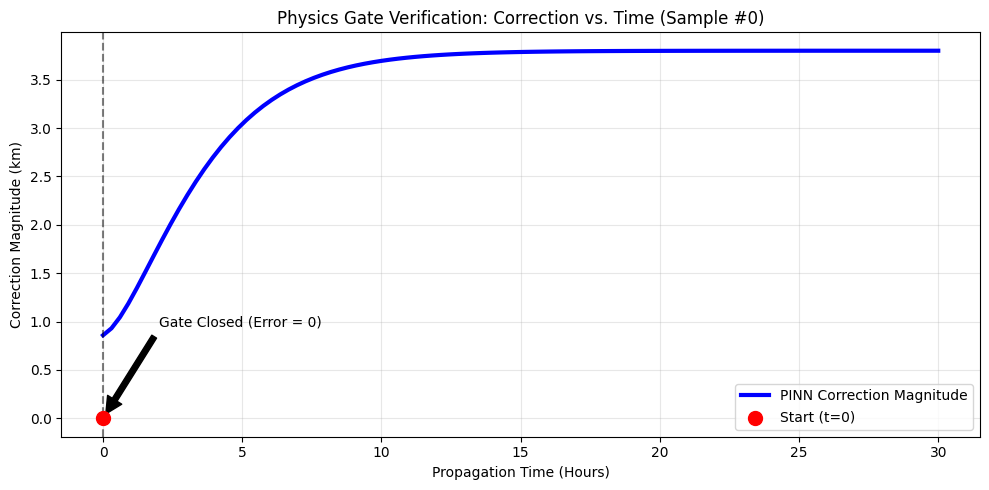
\includegraphics[width=\columnwidth]{figures/gate.png}
\caption{Physics Gate profile $\Gamma(t)=\tanh(\lambda t)$ showing strict suppression near $t=0$.}
\label{fig:physics-gate}
\end{figure}

\begin{figure}[H]
\centering
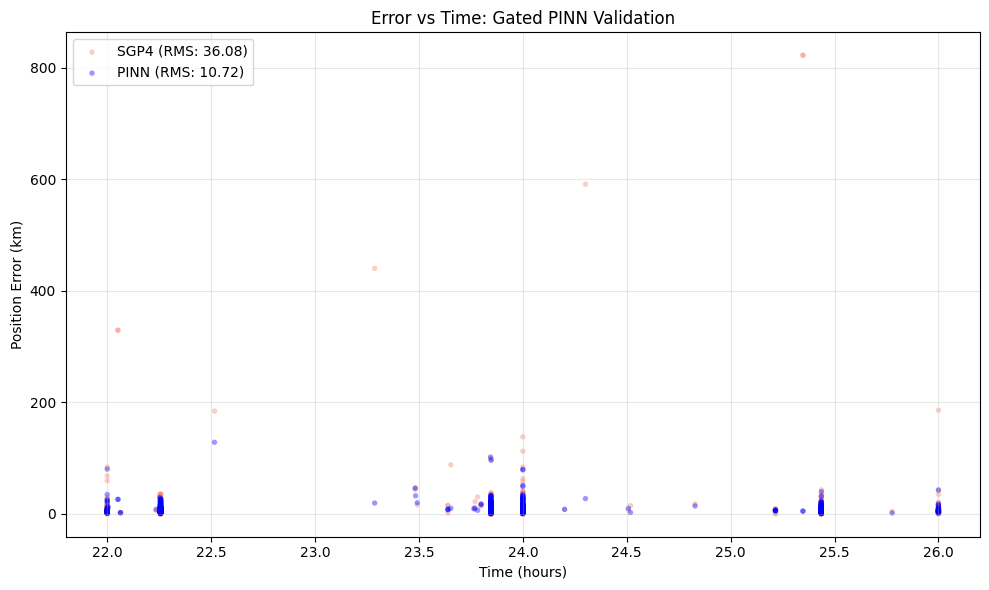
\includegraphics[width=\columnwidth]{figures/pinn_vaidation.png}
\caption{PINN validation performance comparing predicted corrections against held-out samples.}
\label{fig:pinn-validation}
\end{figure}

\subsection{Monte Carlo Conjunction and Mahalanobis Risk}
Operational assessment requires distribution-aware prediction, not only point estimates. We perturb initial states in the RIC frame using anisotropic Gaussian noise,
\begin{equation}
\Sigma_{RIC}=\mathrm{diag}(\sigma_R^2,\sigma_I^2,\sigma_C^2),
\end{equation}
propagate thousands of samples through the G-PINN, and score pairwise encounter risk with Mahalanobis distance:
\begin{equation}
D_M=\sqrt{(\boldsymbol{\mu}_A-\boldsymbol{\mu}_B)^T(\boldsymbol{\Sigma}_A+\boldsymbol{\Sigma}_B)^{-1}(\boldsymbol{\mu}_A-\boldsymbol{\mu}_B)}.
\end{equation}
Risk bands (Critical/Watch/Low) are then assigned from covariance overlap statistics, enabling direct integration with conjunction decision support workflows \cite{sanjuan2021uncertainty,ramesh2025space}.